% \documentclass{article}
% % main document, called main.tex
% \usepackage{tikz}
% 
% \usetikzlibrary{automata,arrows,er,fit,positioning,snakes,shapes,trees}
% 
% 
% \usetikzlibrary{external}
% \tikzexternalize{main} % provide the file’s real name
% \begin{document}
% 
% \begin{tikzpicture} % will b\node {root}
% \node {root}
% child {node {left}}
% child {node {right}
% child {node {child}}
% child {node {child}}
% };
% \end{tikzpicture}
% A simple image is \tikz \fill (0,0) circle(5pt);.
% \end{document}
\documentclass{article}
% main document, called main.tex
\usepackage{tikz}
\usetikzlibrary{external}
\tikzexternalize{main} % provide the file’s real name
\begin{document}
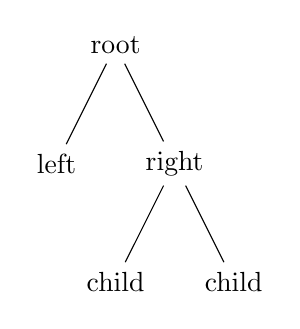
\begin{tikzpicture} % will be written to ’main-figure0.pdf’
\node {root}
child {node {left}}
child {node {right}
child {node {child}}
child {node {child}}
};
\end{tikzpicture}
{
\tikzsetfigurename{subset_}
A simple image is \tikz \fill (0,0) circle(5pt);. %will be written to ’subset_0.pdf’

\begin{tikzpicture} % will be written to ’subset_1.pdf’
\draw[help lines] (0,0) grid (5,5);
\end{tikzpicture}
}% here, the old file name will be restored:
\begin{tikzpicture} % will be written to ’main-figure1.pdf’
\draw (0,0) -- (5,5);
\end{tikzpicture}
\end{document}
